\documentclass[12pt]{report}
\usepackage[utf8]{inputenc}
\usepackage[russian]{babel}
%\usepackage[14pt]{extsizes}
\usepackage{listings}
\usepackage{graphicx}
\usepackage{amsmath,amsfonts,amssymb,amsthm,mathtools} 
\usepackage{pgfplots}
\usepackage{filecontents}
\usepackage{indentfirst}
\usepackage{eucal}
\usepackage{float} 
\usepackage{amsmath}
\usepackage{enumitem}
\usepackage[justification=centering]{caption} 
\usepackage{tikz}
\usepackage{pgfplots}
\pgfplotsset{compat=newest}

\frenchspacing

\usepackage{indentfirst} % Красная строка

\usepackage{listings}
\lstset{
	literate=
	{а}{{\selectfont\char224}}1
	{б}{{\selectfont\char225}}1
	{в}{{\selectfont\char226}}1
	{г}{{\selectfont\char227}}1
	{д}{{\selectfont\char228}}1
	{е}{{\selectfont\char229}}1
	{ё}{{\"e}}1
	{ж}{{\selectfont\char230}}1
	{з}{{\selectfont\char231}}1
	{и}{{\selectfont\char232}}1
	{й}{{\selectfont\char233}}1
	{к}{{\selectfont\char234}}1
	{л}{{\selectfont\char235}}1
	{м}{{\selectfont\char236}}1
	{н}{{\selectfont\char237}}1
	{о}{{\selectfont\char238}}1
	{п}{{\selectfont\char239}}1
	{р}{{\selectfont\char240}}1
	{с}{{\selectfont\char241}}1
	{т}{{\selectfont\char242}}1
	{у}{{\selectfont\char243}}1
	{ф}{{\selectfont\char244}}1
	{х}{{\selectfont\char245}}1
	{ц}{{\selectfont\char246}}1
	{ч}{{\selectfont\char247}}1
	{ш}{{\selectfont\char248}}1
	{щ}{{\selectfont\char249}}1
	{ъ}{{\selectfont\char250}}1
	{ы}{{\selectfont\char251}}1
	{ь}{{\selectfont\char252}}1
	{э}{{\selectfont\char253}}1
	{ю}{{\selectfont\char254}}1
	{я}{{\selectfont\char255}}1
	{А}{{\selectfont\char192}}1
	{Б}{{\selectfont\char193}}1
	{В}{{\selectfont\char194}}1
	{Г}{{\selectfont\char195}}1
	{Д}{{\selectfont\char196}}1
	{Е}{{\selectfont\char197}}1
	{Ё}{{\"E}}1
	{Ж}{{\selectfont\char198}}1
	{З}{{\selectfont\char199}}1
	{И}{{\selectfont\char200}}1
	{Й}{{\selectfont\char201}}1
	{К}{{\selectfont\char202}}1
	{Л}{{\selectfont\char203}}1
	{М}{{\selectfont\char204}}1
	{Н}{{\selectfont\char205}}1
	{О}{{\selectfont\char206}}1
	{П}{{\selectfont\char207}}1
	{Р}{{\selectfont\char208}}1
	{С}{{\selectfont\char209}}1
	{Т}{{\selectfont\char210}}1
	{У}{{\selectfont\char211}}1
	{Ф}{{\selectfont\char212}}1
	{Х}{{\selectfont\char213}}1
	{Ц}{{\selectfont\char214}}1
	{Ч}{{\selectfont\char215}}1
	{Ш}{{\selectfont\char216}}1
	{Щ}{{\selectfont\char217}}1
	{Ъ}{{\selectfont\char218}}1
	{Ы}{{\selectfont\char219}}1
	{Ь}{{\selectfont\char220}}1
	{Э}{{\selectfont\char221}}1
	{Ю}{{\selectfont\char222}}1
	{Я}{{\selectfont\char223}}1
}
\lstset{
	language=Matlab,
	morekeywords={matlab2tikz},
	numbers=left, 
	numberstyle=\tiny,
	stepnumber=1,
	firstnumber=1,
	numbersep=5pt,
	frame=single,
	basicstyle=\footnotesize, 
	showstringspaces=false,
	breaklines=true,
}

%\usetikzlibrary{datavisualization}
%\usetikzlibrary{datavisualization.formats.functions}

\usepackage{amsmath}


% Для листинга кода:
\lstset{ %
	language=haskell,                 % выбор языка для подсветки (здесь это С)
	basicstyle=\small\sffamily, % размер и начертание шрифта для подсветки кода
	numbers=left,               % где поставить нумерацию строк (слева\справа)
	numberstyle=\tiny,           % размер шрифта для номеров строк
	stepnumber=1,                   % размер шага между двумя номерами строк
	numbersep=5pt,                % как далеко отстоят номера строк от подсвечиваемого кода
	showspaces=false,            % показывать или нет пробелы специальными отступами
	showstringspaces=false,      % показывать или нет пробелы в строках
	showtabs=false,             % показывать или нет табуляцию в строках
	frame=single,              % рисовать рамку вокруг кода
	tabsize=2,                 % размер табуляции по умолчанию равен 2 пробелам
	captionpos=t,              % позиция заголовка вверху [t] или внизу [b] 
	breaklines=true,           % автоматически переносить строки (да\нет)
	breakatwhitespace=false, % переносить строки только если есть пробел
	escapeinside={\#*}{*)}   % если нужно добавить комментарии в коде
}

\usepackage[left=2cm,right=2cm, top=2cm,bottom=2cm,bindingoffset=0cm]{geometry}

\usepackage{listings}

\usepackage{titlesec}
\titleformat{\section}
{\normalsize\bfseries}
{\thesection}
{1em}{}
\titlespacing*{\chapter}{0pt}{-30pt}{8pt}
\titlespacing*{\section}{\parindent}{*4}{*4}
\titlespacing*{\subsection}{\parindent}{*4}{*4}
\usepackage{setspace}

\titleformat{\chapter}{\LARGE\bfseries}{\thechapter}{20pt}{\large\bfseries}
\titleformat{\section}{\Large\bfseries}{\thesection}{20pt}{\large\bfseries}

\lstset{extendedchars=\true}

\makeatletter 

\begin{document}
	
%\def\chaptername{} % убирает "Глава"
\thispagestyle{empty}
\begin{titlepage}
	\noindent \begin{minipage}{0.15\textwidth}
		
\includegraphics[width=\linewidth]{pics/logo}
	\end{minipage}
	\noindent\begin{minipage}{0.9\textwidth}\centering
		\textbf{Министерство науки и высшего образования Российской Федерации}\\
		\textbf{Федеральное государственное бюджетное образовательное учреждение высшего образования}\\
		\textbf{~~~«Московский государственный технический университет имени Н.Э.~Баумана}\\
		\textbf{(национальный исследовательский университет)»}\\
		\textbf{(МГТУ им. Н.Э.~Баумана)}
	\end{minipage}
	
	\noindent\rule{18cm}{3pt}
	\newline\newline
	\noindent ФАКУЛЬТЕТ $\underline{\text{«Информатика и системы управления»}}$ \newline\newline
	\noindent КАФЕДРА $\underline{\text{«Программное обеспечение ЭВМ и информационные технологии»}}$\newline\newline\newline\newline\newline
	
	
	\begin{center}
		\noindent\begin{minipage}{1.3\textwidth}\centering
			\Large\textbf{  Отчёт по лабораторной работе №2 по курсу}\newline\newline
			\textbf{<<Математическая статистика>>}\newline
		\end{minipage}
	\end{center}
	
	~\\\\\\\\\\
	\large
	\noindent\textbf{Тема } $\underline{\text{Интвервальные оценки.}}$\newline\newline
	\noindent\textbf{Студент } $\underline{\text{Сироткина П.Ю.}}$\newline\newline
	\noindent\textbf{Номер варианта} $\underline{\text{~~~12~~~}}$\newline\newline
	\noindent\textbf{Группа } $\underline{\text{ИУ7-66Б}}$\newline\newline
	\noindent\textbf{Преподаватель } $\underline{\text{Андреева Т.В.}}$\newline\newline
	\noindent\textbf{Оценка } $\underline{\text{~~~~~~~~~~~~~~~~~~~~~~~~~}}$\newline\newline
	
	\begin{center}
		\vfill
		Москва~---~\the\year
		~г.
	\end{center}
\end{titlepage}

\chapter*{Лабораторная работа №2}

\section*{1. Цель работы}

Построение доверительных интервалов для математического ожидания и дисперсии нормальной случайной величины.

\section*{2. Содержание работы}

\begin{enumerate}
	\item Для выборки объема n из нормальной генеральной совокупности X реализовать в виде программы на ЭВМ:
	\begin{itemize}
		\item Вычисление точечных оценок $\hat\mu(\vec{x_n})$ и $S^2(\vec{x_n}) $ математического ожидания MX и дисперсии DX соответственно;
		\item Вычисление нижней и верхней границ $\underline{\mu}(\vec{x_n})$, $\overline{\mu}(\vec{x_n})$ для $\gamma$-доверительного интервала для математического ожидания MX;
		\item Вычисление нижней и верхней границ $\underline{\sigma}^2(\vec{x_n})$, $\overline{\sigma}^2(\vec{x_n})$ для $\gamma$-доверительного интервала для дисперсии DX.
	\end{itemize}
	\item Вычислить $\hat\mu$ и $S^2$ для выборки из индивидуального варианта;
	\item Для заданного пользователем уровня доверия $\gamma$ и N - объема выборки из индивидуального варианта:
	\begin{itemize}
		\item На координатной плоскости $Oyn$ построить прямую $y = \hat\mu(\vec{x}_N)$, также графики функций $y = \underline{\mu}(\vec{x}_n)$, $y = \overline{\mu}(\vec{x}_n)$ как функций объема выборки, где n изменяется от 1 до N.
		\item На другой координатной плоскости $Ozn$ построить прямую $z = S^2(\vec{x}_N)$, также графики функций $z = \underline{\sigma}^2(\vec{x}_n)$, $z = \overline{\sigma}^2(\vec{x}_n)$ как функций объема выборки, где n изменяется от 1 до N.
	\end{itemize}
\end{enumerate}

\section*{3. Теоретические сведения}

Формулы для вычисления некоторых требуемых величин:

\begin{itemize}
	\item Выборочное среднее: $\hat\mu(\vec{x}) = \overline x = \frac{1}{n} \cdot \sum\limits_{i=1}^{n} x_i$;
	\item Выборочная дисперсия: $S^2(\vec{x}) = \frac{1}{n-1} \cdot \sum\limits_{i=1}^{n} (x_i - \overline x)^2$.
\end{itemize}

\subsection*{Определение $\gamma$-доверительного интервала для значения параметра распределения случайной величины}

Пусть дана случайная величина $X$, закон распределения которой известен с точностью до неизвестного параметра $\theta$.

\textit{Интервальной оценкой} параметра $\theta$ уровня $\gamma$ называют пару статистик $\underline{\theta}(\vec X)$ и $\overline{\theta}(\vec X)$, таких, что $P\{\theta \in (\underline{\theta}(\vec X); \overline{\theta}(\vec X))\} = \gamma.$

$\underline{\theta}(\vec X)$ и $\overline{\theta}(\vec X))\}$ называют верхней и нижней границами интервальной оценки соответственно.

$\gamma$-\textit{доверительным интервалом} для параметра $\theta$ называют реализацию (выборочное значение) интервальной оценки уровня $\gamma$ для этого параметра, т.е. интервал вида ($\underline{\theta}(\vec X); \overline{\theta}(\vec X)$) с детерминированными границами.

\subsection*{Формулы для вычисления границ $\gamma$-доверительного интервала для математического ожидания и дисперсии нормальной случайной величины}

Формулы для вычисления границ $\gamma$-доверительного интервала для математического ожидания:

\begin{equation*}
	\underline{\mu}(\vec{x_n}) = \overline{x} - \frac{S(\vec{x})\cdot t_{\frac{1+\gamma}{2}}}{\sqrt{n}} 
\end{equation*}

\begin{equation*}
	\overline{\mu}(\vec{x_n}) = \overline{x} + \frac{S(\vec{x})\cdot t_{\frac{1+\gamma}{2}}}{\sqrt{n}} 
\end{equation*}

Формулы для вычисления границ $\gamma$-доверительного интервала для дисперсии:

\begin{equation*}
	\underline{\sigma}(\vec{x_n}) = \frac{(n - 1) \cdot S^2(\vec{x})}{h_\frac{1+\gamma}{2}}
\end{equation*}

\begin{equation*}
	\overline{\sigma}(\vec{x_n}) = \frac{(n - 1) \cdot S^2(\vec{x})}{h_\frac{1-\gamma}{2}}
\end{equation*}

Обозначения:

\begin{itemize}
	\item $\overline{x}$ - точечная оценка математического ожидания;
	\item $S^2(\vec{x})$ - исправленная точечная оценка дисперсии;
	\item n - объем выборки;
	\item $\gamma$ - уровень доверия;
	\item $t_\alpha$ - квантиль уровня $\alpha$ распределения Стьюдента с n - 1 степенями свободы (St(n-1));
	\item $h_\alpha$ - квантиль уровня $\alpha$ распределения Хи-квадрат с n - 1 степенями свободы ($\chi^2(n-1)$).
\end{itemize}

\clearpage
\section*{4. Текст программы}

\begin{lstlisting}[language=]
function main()
		pkg load statistics
		X = [11.89, 9.60,  9.29,  10.06, 9.50,  8.93,  9.58,  6.81,  8.69,...
				 9.62,  9.01,  10.59, 10.50, 11.53, 9.94,  8.84,  8.91,  6.90,...
				 9.76,  7.09,  11.29, 11.25, 10.84, 10.76, 7.42,  8.49,  10.10,...
				 8.79,  11.87, 8.77,  9.43,  12.41, 9.75,  8.53,  9.72,  9.45,...
				 7.20,  9.23,  8.93,  9.15,  10.19, 9.57,  11.09, 9.97,  8.81,...
				 10.73, 9.57,  8.53,  9.21,  10.08, 9.10,  11.03, 10.10, 9.47,...
				 9.72,  9.60,  8.21,  7.78,  10.21, 8.99,  9.14,  8.60,  9.14,...
				 10.95, 9.33,  9.98,  9.09,  10.35, 8.61,  9.35,  10.04, 7.85,...
				 9.64,  9.99,  9.65,  10.89, 9.08,  8.60,  7.56,  9.27,  10.33,...
				 10.09, 8.51,  9.86,  9.24,  9.63,  8.67,  8.85,  11.57, 9.85,...
				 9.27,  9.69,  10.90, 8.84,  11.10, 8.19,  9.26,  9.93,  10.15,...
				 8.42,  9.36,  9.93,  9.11,  9.07,  7.21,  8.22,  9.08,  8.88,...
				 8.71,  9.93,  12.04, 10.41, 10.80, 7.17,  9.00,  9.46,  10.42,...
				 10.43, 8.38,  9.01]
		
		% Уровень доверия
		gamma = 0.9;
		%gamma = input('Введите уровень доверия: ')
		% Объем выборки 
		N = length(X);
		% Точечная оценка мат. ожидания
		M = mean(X);
		% Точечная оценка дисперсии
		S2 = var(X);
		% Нижняя граница доверительного интервала для мат. ожидания
		M_low = find_m_low(N, M, S2, gamma);
		% Верхняя граница доверительного интервала для мат. ожидания
		M_high = find_m_high(N, M, S2, gamma);
		% Нижняя граница доверительного интервала для дисперсии
		S2_low = find_S2_low(N, S2, gamma);
		% Верхняя граница доверительного интервала для дисперсии
		S2_high = find_S2_high(N, S2, gamma);
		
		% Вывод полученных ранее значений
		fprintf('Точечная оценка математического ожидания = %.3f\n', M);
		fprintf('Точечная оценка дисперсии = %.3f\n', S2);
		fprintf('Нижняя граница доверительного интервала для математического ожидания = %.3f\n', M_low);
		fprintf('Верхняя граница доверительного интервала для математического ожидания = %.3f\n', M_high);
		fprintf('Нижняя граница доверительного интервала для дисперсии = %.3f\n', S2_low);
		fprintf('Верхняя граница доверительного интервала для дисперсии = %.3f\n', S2_high);
		
		% Массив точечных оценок для математического ожидания
		M_array = zeros(1, N)
		% Массив точечных оценок для дисперсии
		S2_array = zeros(1, N)
		% Массивы для нижних и верхних границ для математического ожидания
		M_low_array = zeros(1, N)
		M_high_array = zeros(1, N)
		% Массивы для нижних и верхних границ для дисперсии
		S2_low_array = zeros(1, N)
		S2_high_array = zeros(1, N)
		
		for i = 1 : N
		temp_m = mean(X(1:i));
		temp_s2 = var(X(1:i));
		M_array(i) = temp_m;
		S2_array(i) = temp_s2;
		M_low_array(i) = find_m_low(i, temp_m, temp_s2, gamma);
		M_high_array(i) = find_m_high(i, temp_m, temp_s2, gamma);
		S2_low_array(i) = find_S2_low(i, temp_s2, gamma);
		S2_high_array(i) = find_S2_high(i, temp_s2, gamma);
		end
		
		% Построение графиков
		plot(1 : N, [(zeros(1, N) + M)', M_array', M_low_array', M_high_array']);
		xlabel('n');
		ylabel('y');
		legend('f1', 'f2', 'f3', 'f4');
		
		figure;
		
		plot(1 : N, [(zeros(1, N) + S2)', S2_array', S2_low_array', S2_high_array']);
		xlabel('n');
		ylabel('z');
		legend('g1', 'g2', 'g3', 'g4');
end
	
% Функция поиска нижней границы доверительного интервала для математического ожидания
function M_low = find_m_low(N, M, S2, gamma)
	M_low = M - sqrt(S2) * tinv((1 + gamma) / 2, N - 1) / sqrt(N);
end
% Функция поиска верхней границы доверительного интервала для математического ожидания
function M_high = find_m_high(N, M, S2, gamma)
	M_high = M + sqrt(S2) * tinv((1 + gamma) / 2, N - 1) / sqrt(N);
end
% Функция поиска нижней границы доверительного интервала для дисперсии
function S2_low = find_S2_low(N, S2, gamma)
	S2_low = ((N - 1) * S2) / chi2inv((1 + gamma) / 2, N - 1);
end
% Функция поиска верхней границы доверительного интервала для дисперсии
function S2_high = find_S2_high(N, S2, gamma)
	S2_high = ((N - 1) * S2) / chi2inv((1 - gamma) / 2, N - 1);
end
\end{lstlisting}

\section*{5. Результат расчетов и графики для выборки из индивидуального варианта (при построении графиков принять $\gamma$ = 0.9)}

\begin{itemize}
	\item $\hat \mu (\vec x_n) = 9.487$;
	\item $ S^2 (\vec x_n) = 1.217$;
	\item $\underline \mu (\vec x_n) = 9.320$;
	\item $\overline\mu (\vec x_n) = 9.654$
	\item $\underline \sigma (\vec x_n) = 0.996$;
	\item $\overline \sigma (\vec x_n) = 1.528$
\end{itemize}

Обозначения на графиках:

\begin{itemize}
	\item f1: $y(n) = \hat\mu(\vec x_N)$;
	\item f2: $y(n) = \underline\mu(\vec x_n)$;
	\item f3: $y(n) = \overline\mu(\vec x_n)$;
	\item f4: $y(n) = \mu(\vec x_n)$;
\end{itemize}
~\
\begin{itemize}
	\item g1: $z(n) = S^2(\vec x_N)$;
	\item g2: $z(n) = \underline \sigma^2(\vec x_n)$;
	\item g3: $z(n) = \overline \sigma^2(\vec x_n)$;
	\item g4: $z(n) = \sigma^2(\vec x_n)$.
\end{itemize}

\begin{figure}[!h]
	\center{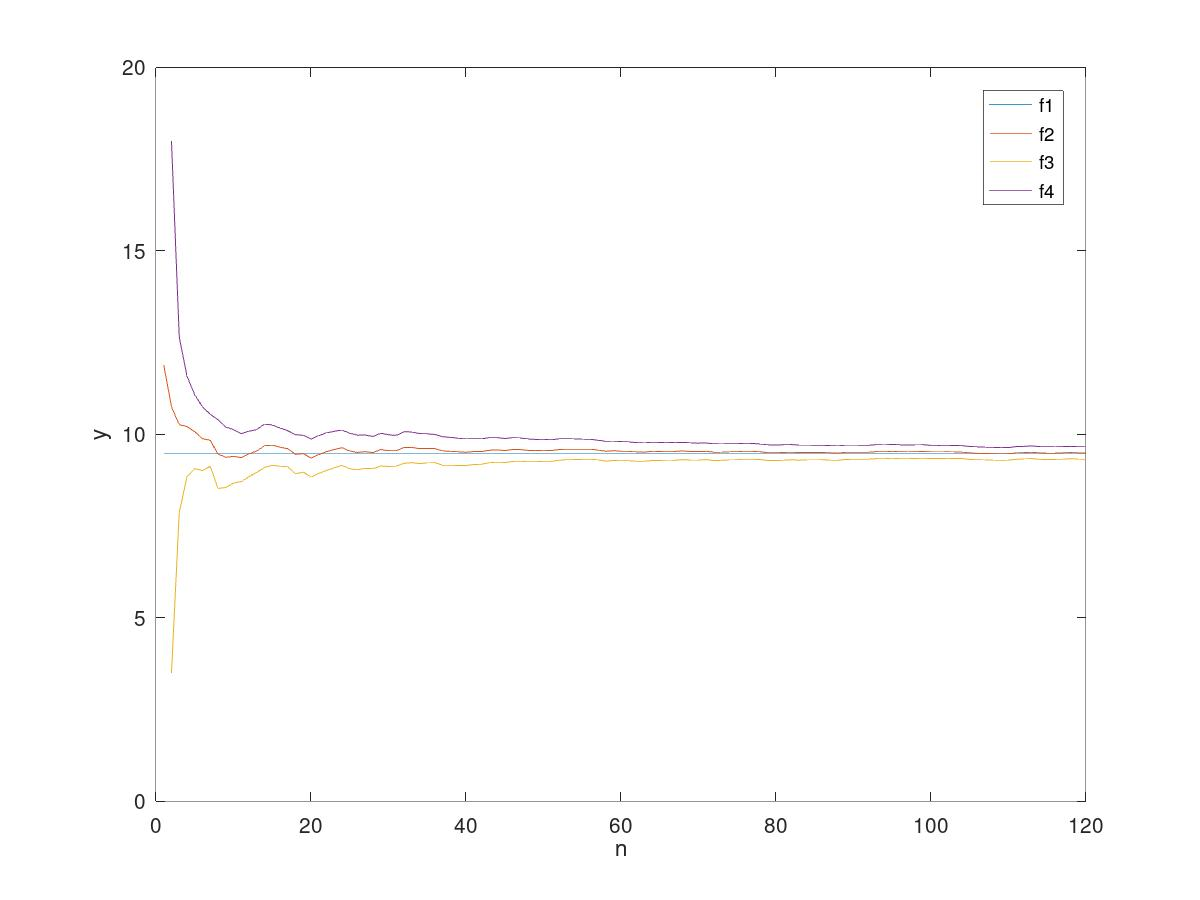
\includegraphics[scale=0.45]{pics/p1.jpg}}
	\caption{Прямая $y(n) = \hat\mu(\vec x_N)$, а также графики функций $y(n) = \underline\mu(\vec x_n)$, $y(n) = \overline\mu(\vec x_n)$, $y(n) = \mu(\vec x_n)$ как функций объема $n$ выборки, где $n$ изменяется от 1 до $N$}
\end{figure}

\begin{figure}[!h]
	\center{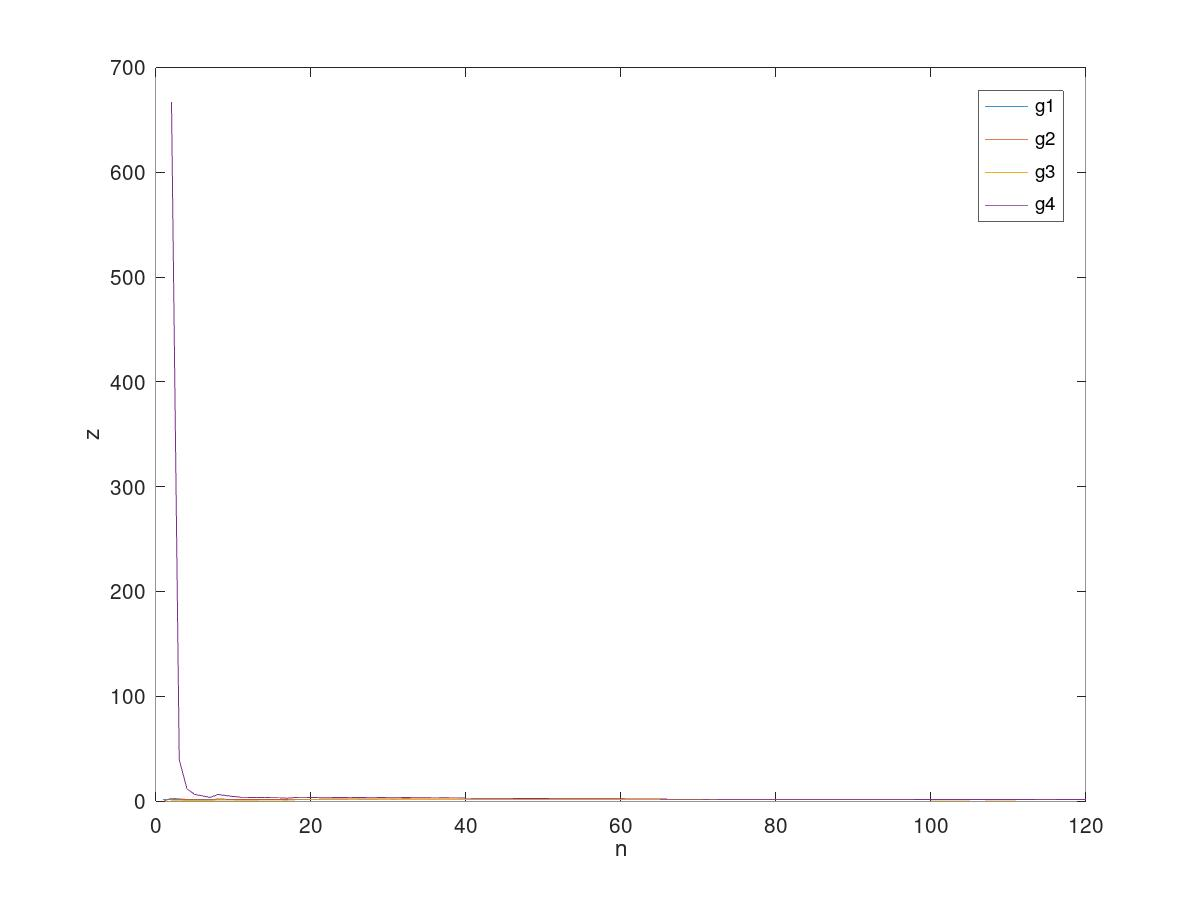
\includegraphics[scale=0.45]{pics/p2.jpg}}
	\caption{Прямая $z(n) = S^2(\vec x_N)$, а также графики функций $z(n) = \underline \sigma^2(\vec x_n)$, $z(n) = \overline \sigma^2(\vec x_n)$, $z(n) = \sigma^2(\vec x_n)$ как функций объема $n$ выборки, где $n$ изменяется от 1 до $N$}
\end{figure}

\begin{figure}[!h]
	\center{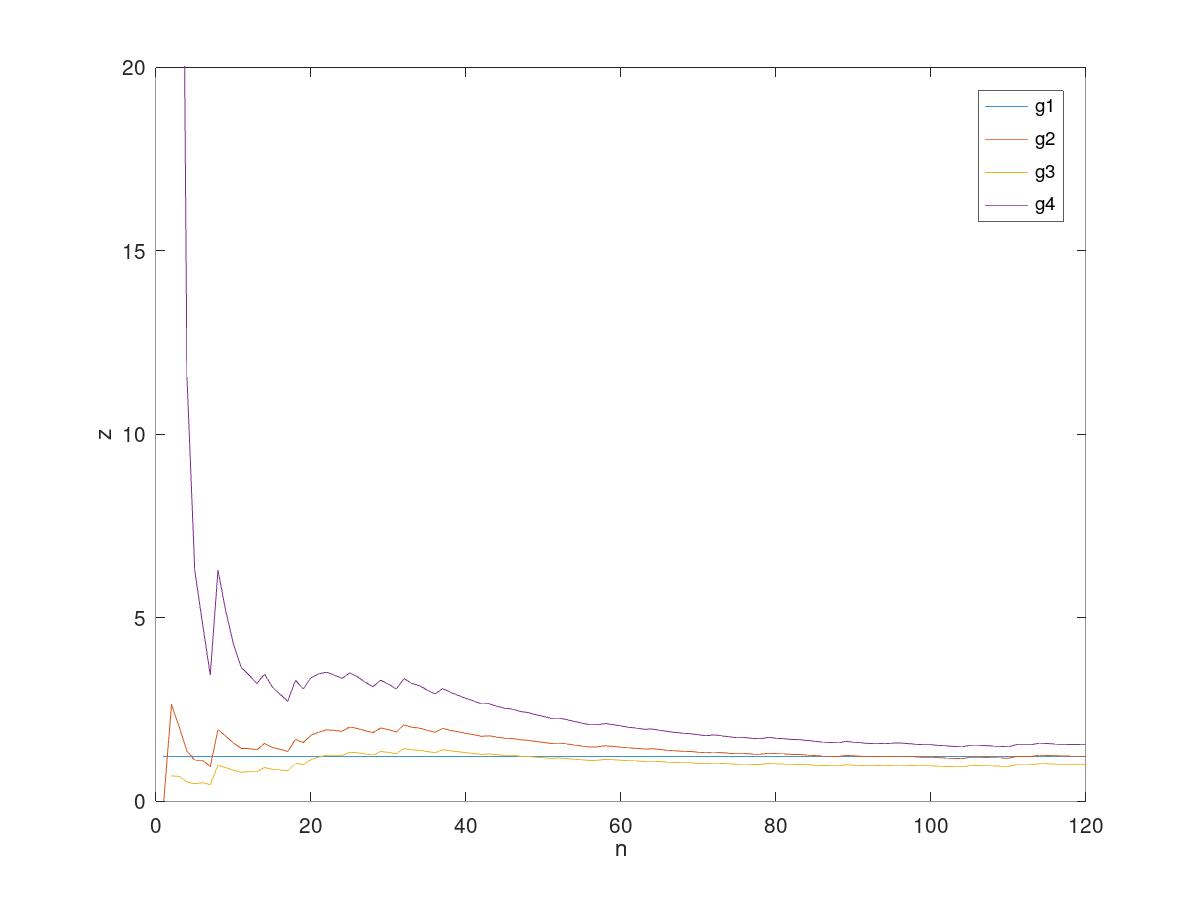
\includegraphics[scale=0.45]{pics/p2s.jpg}}
	\caption{Прямая $z(n) = S^2(\vec x_N)$, а также графики функций $z(n) = \underline \sigma^2(\vec x_n)$, $z(n) = \overline\sigma^2(\vec x_n)$, $z(n) = \sigma^2(\vec x_n)$ как функций объема $n$ выборки, где $n$ изменяется от 1 до $N$ (приближенный к началу координат график)}
\end{figure}

\end{document}